\documentclass{beamer}
\usepackage[utf8]{inputenc}
\usetheme{metropolis} 
\usepackage{listings}
%\usepackage[backend=biber, style=numeric, doi=false,isbn=false,url=false, giveninits=true]{biblatex}
%\usepackage{biblatex}
\usepackage[backend=biber]{biblatex}
%\usepackage[backend=bibtex]{biblatex}
\usepackage{hyperref}
\usepackage{booktabs} % Required for better horizontal rules in tables
\usepackage{multirow}
\usepackage{multicol}

\lstset{
	sensitive=false,    % not case-sensitive
	morecomment=[l]{;;}, % line comment
	alsoletter={:,-},   % consider extra characters
	frame=single,
	numbers=left,
	breaklines=true,
	tabsize=2,
	basicstyle=\tiny,
}


%\usepackage[
%backend=biber,
%style=alphabetic,
%citestyle=numeric
%]{biblatex}

%\setbeamertemplate{bibliography item}{\insertbiblabel}


\addbibresource{bibliography.bib}

\title{Planning and Scheduling  @home project}
\date{\today}
\author{\'{A}ngela Patricia Enr\'{i}quez G\'{o}mez \\ Ethan Oswald Massey \\ Maximilian Mensing}
\institute{BRSU}
\begin{document}
	\maketitle
	
	\begin{frame}{\textsl{Stroring Groceries}}
		
		\begin{itemize}
			\item \textbf{Problem 1}: The table and the cupboard are located and known. The cupboard door is closed. One object is on the table and has to be placed on any shelf. 
			\item \textbf{Problem 2}: The table and the cupboard have to be located. The cupboard door is closed. There are $n$ \footnote{$n$ is between 2 and 5} known objects on the table. The objects have to be placed on any shelf.
			\item \textbf{Problem 3}: As case 2 except for - The objects are not known (perception has to be used).
			
			\item \textbf{Problem 4}: As case 3 except for - Each shelf holds objects of one category (the cupboard has to be explored). Place each object on the correct shelf according to the category.
			
		\end{itemize}
		
	\end{frame}
	
	\begin{frame}{\textsl{Selection of the Planner}}
		
		\textbf{SHOP2 (Simple Hierarchical Ordered Planner)}.
		
		\begin{itemize}
			\item Uses partial-order forward decomposition. 
			\item The knowledge base is easier to build than with SHOP.
			\item Methods allow a list of preconditions which are evaluated in order of appearance.
			\item Simplicity in the representation of methods and operators.
		\end{itemize} 
		
	\end{frame}	
	
	\begin{frame}
		
		\begin{figure}
			\centering
			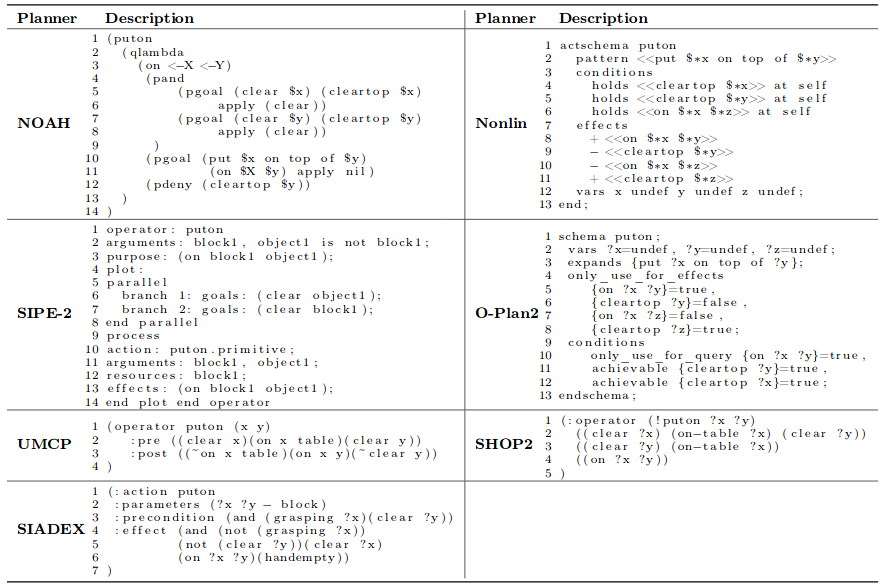
\includegraphics[width=1\linewidth]{../Report/images/jshop}
			\caption{$put-on$ operator for HTN planners \cite{Georgievski2014}}
			\label{fig:jshop}
		\end{figure}
		
	\end{frame}
	
	\begin{frame}{\textsl{Using JSHOP2}}
		\begin{itemize}
			\item Get jshop from: \url{https://github.com/mas-group/jshop2}
			\item Set environment: \textbf{ \small export CLASSPATH="`pwd`/bin.build/JSHOP2.jar:`pwd`/antlr.jar:."}
			\item Compile: \textbf{{\small make c}}
			\item Run:
			\begin{itemize}
				\item \textbf{\small make problem1} 
				\item \textbf{\small make problem2}
				\item \textbf{\small make problem3} 
				\item \textbf{\small make problem4}
			\end{itemize} 

		\end{itemize}
		
	\end{frame}
	
	\begin{frame}{Modeling the domain}
		\begin{itemize}
			\item Includes:
			\begin{itemize}
				\item Operators: Directly perform primitive tasks. Use preconditions, delete and add lists.
				\item Methods: Decompose compound tasks into other compound or primitive tasks. Use preconditions and task lists.
				\item Axioms: Map meaning of symbols.
			\end{itemize}
		\end{itemize}
		
		\begin{table}[h!]
			
			\centering
			\scriptsize
			
			\begin{tabular}{cl}
				\toprule
				
				Problem & Compound task to achieve \\
				\midrule
				
				1 & mode-known-object ?a ?t ?c ?s \\
				
				\midrule
				
				2 & move-known-objects ?t ?c ?s ?tray \\
				
				\midrule
				
				3 & move-uncategorized-objects ?t ?c ?s ?tray ?camera \\
				
				\midrule
				
				4 & move-unlabeled-object-unknown-cupboard ?t ?c ?s ?tray ?camera \\
				
				\bottomrule
			\end{tabular}
			\caption{Tasks to achieve for problems 1 to 4.}
			\label{table:compund-tasks}
		\end{table}
		
	\end{frame}
	
	\begin{frame}{Assumptions}
			
			%Common sense assumptions were made to limit domain complexity.
		
			%\item Assumptions include, but are not limited to:
			\begin{itemize}
				\item There is exactly the number of objects required (e.g. only one table).
				\item The initial position of the robot is at the table.
				\item The robot is able to sense and identify all objects correctly.
				\item All objects placed on the table should be stored on the shelves.
				\item The robot uses a tray of infinite capacity to carry objects.
				\item Each shelf initially holds an object and there is one shelf per object category (problem 4).
				
			\end{itemize}
			%\item Testing began with the smallest domain (Problem 1) and gradually increase in complexity

	\end{frame}
	
	
	\begin{frame}{Defining the problem}
		\begin{itemize}
			\item A problem file is created for each problem.
			\item The problem file contains the initial state and the compound task to be solved.
			\item HTN planner uses the problem file and the domain to create a solution.
		\end{itemize}
	\end{frame}
	
	%\begin{frame}{Problem 1}
	
		
\begin{lstlisting}
(defproblem problem1 storegroceries
;;Problem 1
(
(object a1)
(cupboard c1)
(door d1)
(shelf s1)
(table t1)
(robot r1)
(on a1 t1) (door-closed d1)(robot-at r1 t1)
)
((move-known-object a1 t1 c1 s1))
)
\end{lstlisting}
	
		\textbf{Problem 1.}The table and the cupboard are located and known. The cupboard door is closed. One object is on the table and has to be placed on any shelf. \vspace{7cm}
		
		
		\textbf{                                                     }
		\textbf{                                                     }
		\textbf{                                                     }
		\textbf{                                                     }
		\textbf{                                                     }
		\textbf{                                                     }

		
	The task is decomposed using the method $move-known-object ?a ?t ?c ?s$
	
	\begin{lstlisting}
	(:method (move-known-object ?a ?t ?c ?s)
	branch1
	((robot-at ?r ?t)(on ?a ?t)(door-open ?d))
	((!pickup ?a ?t)(!move ?r ?t ?c)(!putdown ?a ?s))
	
	branch2
	((robot-at ?r ?t)(on ?a ?t)(door-closed ?d))
	((!move ?r ?t ?c)(!open-door ?d)(!move ?r ?c ?t)(!pickup ?a ?t)(!move ?r ?t ?c)(!putdown ?a ?s)))
	\end{lstlisting}

	
	\begin{frame}{GUI Result}
		\begin{figure}[h!]
			\centering
			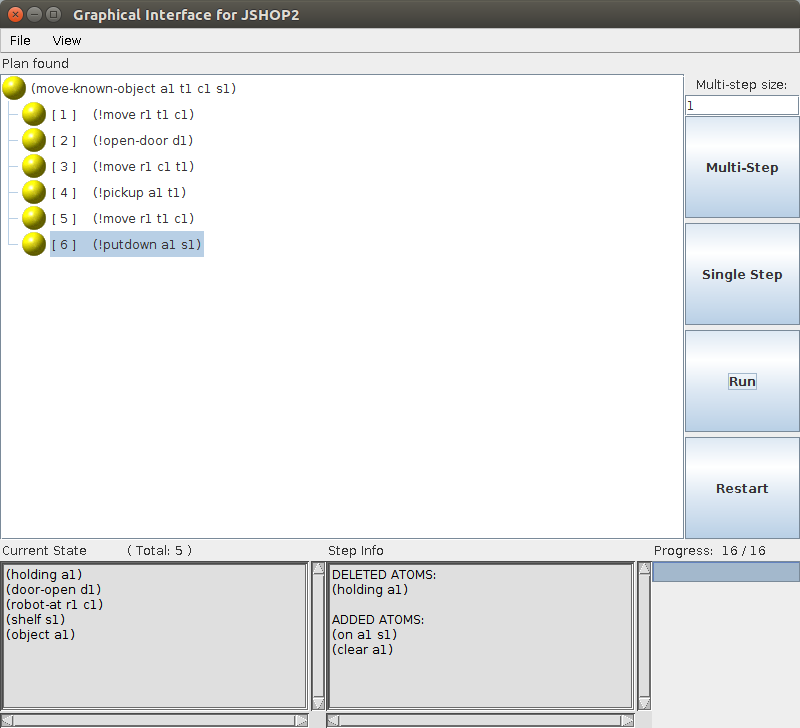
\includegraphics[width=0.7\linewidth]{images/problem1_gui}
			\caption{Solution problem 1.}
			\label{fig:probem1_gui}
		\end{figure}
	\end{frame}
	
	
	\begin{frame}
		\textbf{Problem 4.} The table and the cupboard have to be located. The cupboard door is closed. There are $n$ \footnote{$n$ is between 2 and 5} unknown objects on the table. Each shelf holds objects of one category (the cupboard has to be explored). Place each object on the correct shelf according to the category.
			
	\end{frame}
	
\begin{lstlisting}
(defproblem problem4 storegroceries
;;Problem4 with 2 objects
(
(object a1)
(object a2)
(camera camera1)
(cupboard c1)
(door d1)
(shelf s1)
(shelf s2)
(shelf s3)
(table t1)
(robot r1)
(tray tray1)

(unknown-location t1)(unknown-location c1)(unlabeled c1)
(holds-snack s1)
(holds-drink s2)
(holds-fruit s3)
(on a1 t1)(is-bag a1)(is-crunchy a1)
(on a2 t1)(is-bottle a2)
(door-closed d1)(robot-at r1 t1)
)
((move-unlabeled-object-unknown-cupboard t1 c1 s1 tray1 camera1))
)
\end{lstlisting}

\textbf{                                }
\textbf{                                }
\textbf{                                }




\begin{lstlisting}
[ 1 ]    (!locate t1)
[ 2 ]    (!locate c1)
[ 3 ]    (!move r1 t1 c1)
[ 4 ]    (!open-door d1)
[ 5 ]    (!label-shelf s1)
[ 6 ]    (!label-shelf s2)
[ 7 ]    (!label-shelf s3)
[ 8 ]    (!move r1 c1 t1)
[ 9 ]    (!label-object a1)
[ 10 ]    (!label-object a2)
[ 11 ]    (!pickup a1 t1)
[ 12 ]    (!putdown a1 tray1)
[ 13 ]    (!pickup a2 t1)
[ 14 ]    (!putdown a2 tray1)
[ 15 ]    (!move r1 t1 c1)
[ 16 ]    (!pickup a1 tray1)
[ 17 ]    (!putdown a1 s1)
[ 18 ]    (!pickup a2 tray1)
[ 19 ]    (!putdown a2 s2)
\end{lstlisting}

	
	\begin{frame}
			Table \ref{table:n-objects} compares the number of steps for generating plans for problems 2, 3 and 4 and the number of tasks in the plan, when the number of objects is 2, 3, 4 and 5.
			
	\begin{table}[h!]
		
		\centering
		\scriptsize
		
		\begin{tabular}{cccc}
			\toprule
			
			Problem & Objects & Steps  & Primitive tasks\\
			\midrule
			
			\multirow{3}{*}[-3pt]{2} & {2} & {46} & {14} \\
			
			{} & {3} & {58} & {18} \\
			
			{} & {4} & {70} & {22} \\
			
			{} & {5} & {82} & {26} \\
			
			\midrule
			
			\multirow{3}{*}[-3pt]{3} & {2} & {56} & {16} \\
			
			{} & {3} & {72} & {21} \\
			
			{} & {4} & {88} & {26} \\
			
			{} & {5} & {104} & {31} \\
			
			\midrule
			
			\multirow{3}{*}[-3pt]{4} & {2} & {70} & {19} \\
			
			{} & {3} & {86} & {24} \\
			
			{} & {4} & {102} & {29} \\
			
			{} & {5} & {118} & {34} \\
			
			\bottomrule
		\end{tabular}
		\caption{Number of steps and tasks for plans with $n$ objects.}
		\label{table:n-objects}
	\end{table}
			
	\end{frame}
	
	
	\begin{frame}{Limitations}
		\begin{itemize}
			\item Without sufficient prior information the planner is not able to classify objects.
			\item If assumptions are invalidated the planner will fail.
			\item In problem 4, if the shelves don't have example objects the planner does not know where to store the objects.
			\item Executing with java -ra generates all possible plans.
			\begin{itemize}
				\item High space and time complexity.
				\item Maximum of 4 objects to avoid outOfMemoryError.
			\end{itemize}
		\end{itemize}
	\end{frame}
	
	\begin{frame}{The planner does not have information for classifying an object.}
			If the information needed for classifying an object is missing from the problem definition, the object will no be classified and the planner will get stuck in the recursion of the method $label-objects$. 
			
	\end{frame}
			
		\begin{lstlisting}
	 ;; To label the objects
	 (:method (label-objects)
	 branch1
	 (forall (?z) ((object ?z))(labeled ?z))
	 nil
	 
	 branch2
	 ((object ?z)(not (labeled ?z)))
	 ((!label-object ?z)(label-objects))
	 )
		\end{lstlisting}
		
		Figure \ref{fig:failure-1} shows the output of the planner when 6 objects are in the problem definition and the information for classifying one of them is missing. The planner runs 17715 steps but fails to return a plan because the information about object $a4$ is missing. All objects should be labeled to stop the recursion. Since this condition is never met, the plan fails. \\
		
		\begin{frame}
		
		\begin{figure} [ht!]
			\centering
			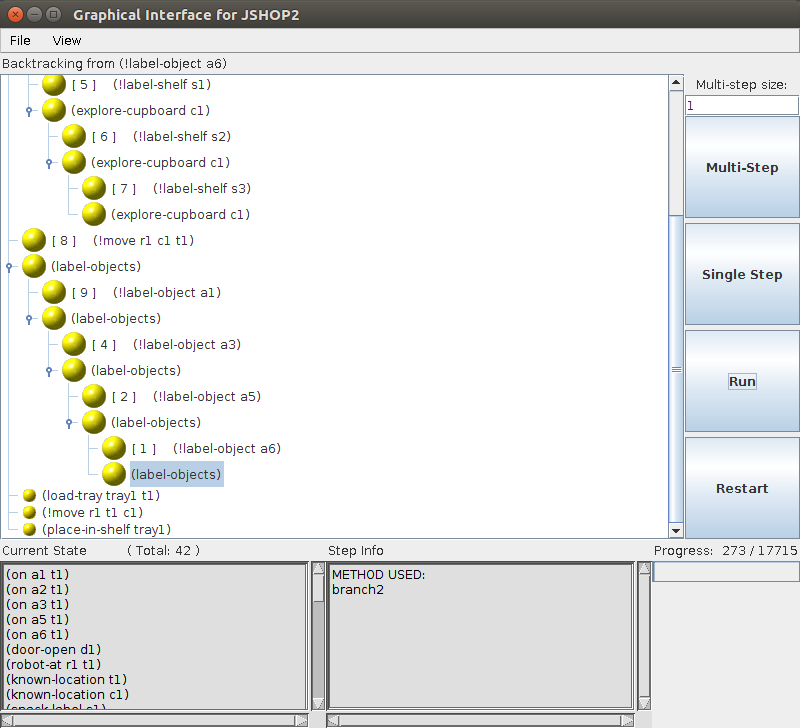
\includegraphics[width=0.7\linewidth]{images/failure-1}
			\caption{Failure: The planner does not have enough information for classifying an object.}
			\label{fig:failure-1}
		\end{figure}
		
		\end{frame}
		


%\begin{frame}
%	\printbibliography
	
%\end{frame}




\end{document}